\documentclass[11pt]{article}
% Time-stamp: <homework-02.tex, saved on Fri, Sep 14, 2007 at 12:46pm>
\usepackage[margin=1in, head=1in]{geometry}
\usepackage{amsmath, amssymb, amsthm}
\usepackage{fancyhdr}
\usepackage{graphicx}
\usepackage{pgfplots}

%\usepackage{pdfsync}
\addtolength{\textwidth}{.5in}
\addtolength{\leftmargin}{-1in}
\addtolength{\textheight}{.5in}
\addtolength{\topmargin}{-0.5in}

%\pagestyle{fancy}
%\lhead{MATH 200X }
%\chead{Fall 2007}
%\rhead{FINAL EXAM}
%\lfoot{}
%\cfoot{\thepage}
%\rfoot{}

\setcounter{secnumdepth}{0}
%\renewcommand{\theenumi}{\alph{enumi}}
%\renewcommand{\emptyset}{\varnothing}
\newcommand{\R}{\mathbb{R}}
\newcommand{\N}{\mathbb{N}}
\newcommand{\Z}{\mathbb{Z}}
\newcommand{\clm}{\par\textit{Claim:}\par}
\newcommand{\diam}{\mathrm{diam}}
\newcommand{\sect}{\textsection}

\parindent=0in
\parskip=0.5\baselineskip

\begin{document} 

\begin{center}MATH 156: Precalculus  \\ Fall 2015 \\ Worksheet \sect 2.3: Getting Information from the Graph of a Function\end{center}

\hrulefill

{\sc{Introduction}}

Definition: A function is {\bf{increasing}} on an interval $I$ if \\
\begin{center} \fbox{ \begin{minipage}{2in} \hfill\vspace{0.3in} \end{minipage} }  whenever $x_1 < x_2$ in $I$. \end{center}
A function is {\bf{increasing}} on an interval $I$ if \\

\begin{center} \fbox{ \begin{minipage}{2in} \hfill\vspace{0.3in} \end{minipage} }  whenever $x_1 < x_2$ in $I$. \end{center}

Examples:

\begin{tabular}{ccc}
$y=x^2$ & $y=x^3$ & $y=1/x$\\
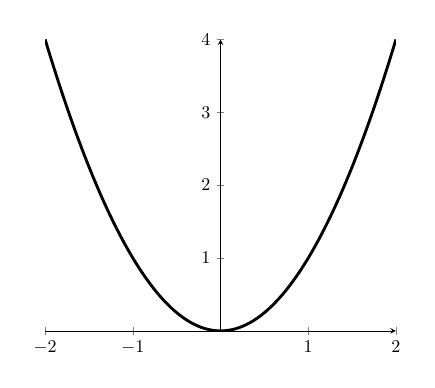
\begin{tikzpicture}[scale=0.65]
\begin{axis}[
        axis x line=middle, 
        axis y line=middle, 
        ]
    \addplot[domain=-2:2, samples=400, black, ultra thick]  {x^2};
 \end{axis}
\end{tikzpicture}
&
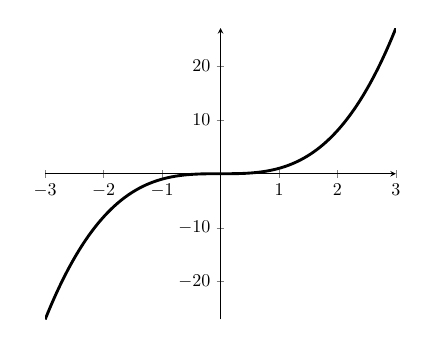
\begin{tikzpicture}[scale=0.65]
\begin{axis}[
        axis x line=middle, 
        axis y line=middle, 
        ]
    \addplot[domain=-3:3, samples=400, black, ultra thick]  {x^3};
 \end{axis}
\end{tikzpicture}
&
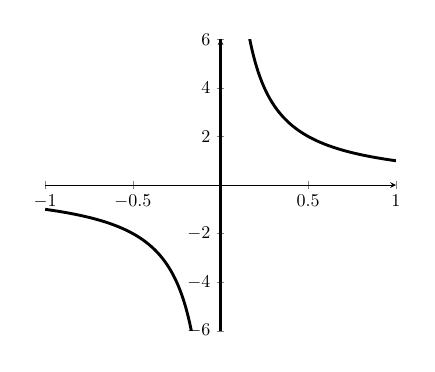
\begin{tikzpicture}[scale=0.65]
\begin{axis}[
        axis x line=middle, 
        axis y line=middle, 
        ymax=6, 
        ymin=-6
        ]
    \addplot[domain=-1:1, samples=400, black, ultra thick]  {1/x};
 \end{axis}
\end{tikzpicture}\\

\end{tabular}

Definition: A function $f$ has a {\bf{local maximum}} at $x=c$ if \fbox{ \begin{minipage}{2in} \hfill\vspace{0.3in} \end{minipage} } when $x$ is near $c.$\\
A function $f$ has a {\bf{local minimum}} at $x=c$ if \fbox{ \begin{minipage}{2in} \hfill\vspace{0.3in} \end{minipage} } when $x$ is near $c.$\\

Example: $f(x)=x^4+x^3-11x^2-9x+18$ \\
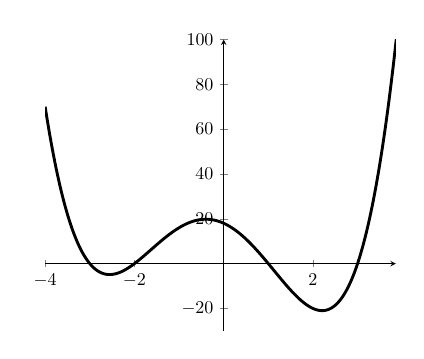
\begin{tikzpicture}[scale=0.65]
\begin{axis}[
        axis x line=middle, 
        axis y line=middle, 
        ymax=100, 
        ymin=-30
        ]        
    \addplot[domain=-4:4, samples=400, black, ultra thick]  {x^4+x^3-11*x^2-9*x+18};
 \end{axis}
\end{tikzpicture}\\
 \newpage
 

{\sc{Try Yourself}} For each graph, (i) determine the domain, range, (ii) identify the open intervals where the function is increasing, decreasing or constant, and (iii) estimate the $x$-values of any local maximums or minimums.\\
NOTE: These are all graphed by a COMPUTER! You need to use your own judgement about the correctness of the computer's image.\\

\begin{tabular}{ccc|ccc}
%row1
$f(x) = \frac{3}{2}x$ & 
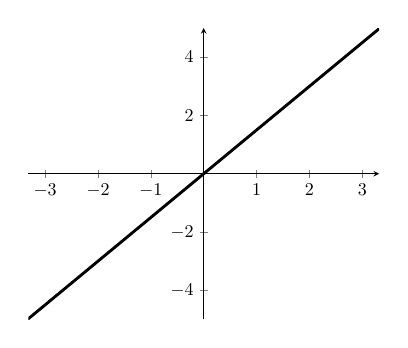
\begin{tikzpicture}[scale=0.65]
\begin{axis}[
        axis x line=middle, 
        axis y line=middle, 
        ymax=5, 
        ymin=-5
        ]        
    \addplot[domain=-4:4, samples=400, black, ultra thick]  {3*x/2};
 \end{axis}
\end{tikzpicture}
&&&
$f(x)=x^2-4x$
&
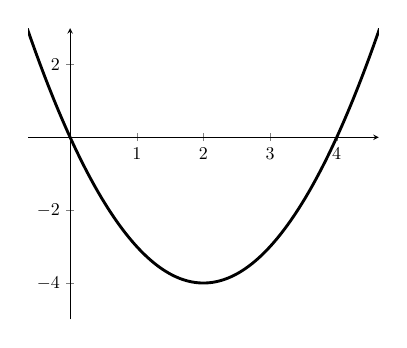
\begin{tikzpicture}[scale=0.65]
\begin{axis}[
        axis x line=middle, 
        axis y line=middle, 
        ymax=3, 
        ymin=-5
        ]        
    \addplot[domain=-4:8, samples=400, black, ultra thick]  {x^2-4*x};
 \end{axis}
\end{tikzpicture} \\
&&&&&\\
\hline
%row2
$f(x) = x^3-3x^2+2$ & 
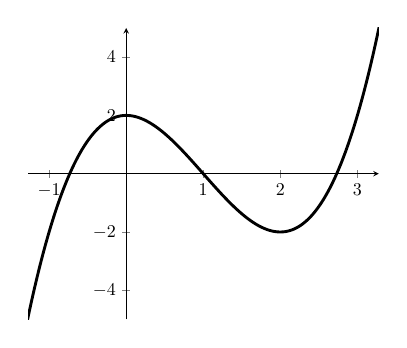
\begin{tikzpicture}[scale=0.65]
\begin{axis}[
        axis x line=middle, 
        axis y line=middle, 
        ymax=5, 
        ymin=-5
        ]        
    \addplot[domain=-4:4, samples=400, black, ultra thick]  {x^3-3*x^2+2};
 \end{axis}
\end{tikzpicture}
&&&
$f(x)=\sqrt{x^2-1}$
&
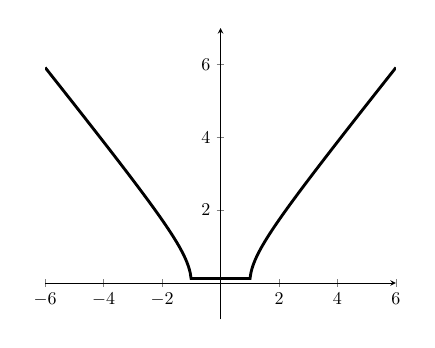
\begin{tikzpicture}[scale=0.65]
\begin{axis}[
        axis x line=middle, 
        axis y line=middle, 
        ymax=7, 
        ymin=-1
        ]        
    \addplot[domain=-6:6, samples=400, black, ultra thick]  {(x^2-1)^(1/2)};
 \end{axis}
\end{tikzpicture} \\
&&&&&\\
\hline
%row3
$f(x) = 3$ & 
\begin{tikzpicture}[scale=0.65]
\begin{axis}[
        axis x line=middle, 
        axis y line=middle, 
        ymax=5, 
        ymin=-5
        ]        
    \addplot[domain=-4:4, samples=400, black, ultra thick]  {3};
 \end{axis}
\end{tikzpicture}
&&&
$f(x)=x^{2/3}$
&
\begin{tikzpicture}[scale=0.65]
\begin{axis}[
        axis x line=middle, 
        axis y line=middle, 
        ymax=7, 
        ymin=-1
        ]        
    \addplot[domain=-6:6, samples=400, black, ultra thick]  {((x)^(1/3))^2};
 \end{axis}
\end{tikzpicture} \\
&&&&&\\
\hline
%row4
$f(x) = -x^{3/4}$ & 
\begin{tikzpicture}[scale=0.65]
\begin{axis}[
        axis x line=middle, 
        axis y line=middle, 
        title={$f(x) = -x^{3/4}$},
        ymax=5, 
        ymin=-5
        ]        
    \addplot[domain=-4:4, samples=400, black, ultra thick]  {(-1)*x^(3/4)};
 \end{axis}
\end{tikzpicture}
&&&
$f(x)=x\sqrt{x+3}$
&
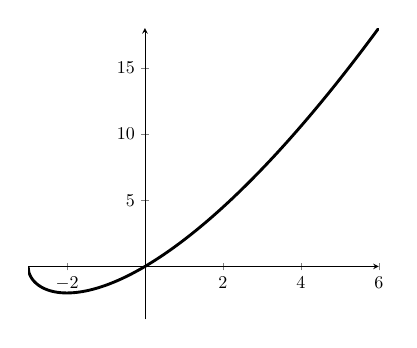
\begin{tikzpicture}[scale=0.65]
\begin{axis}[
        axis x line=middle, 
        axis y line=middle, 
        %ymax=7, 
        ymin=-4
        ]        
    \addplot[domain=-3:6, samples=400, black, ultra thick]  {x*(x+3)^(1/2)};
 \end{axis}
\end{tikzpicture} \\
\end{tabular}
\newpage

\begin{tabular}{ccc}
%row5
$f(x) = \vert x+1\vert+\vert x-1 \vert $ & \hspace{1in} &$f(x)=-\vert x+4 \vert - \vert x+1 \vert$\\
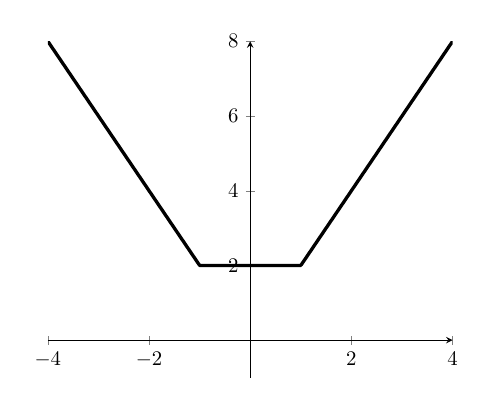
\begin{tikzpicture}[scale=0.75]
\begin{axis}[
        axis x line=middle, 
        axis y line=middle, 
        %ymax=5, 
        ymin=-1
        ]        
    \addplot[domain=-4:4, samples=400, black, ultra thick]  {abs(x+1)+abs(x-1)};
 \end{axis}
\end{tikzpicture}
&&
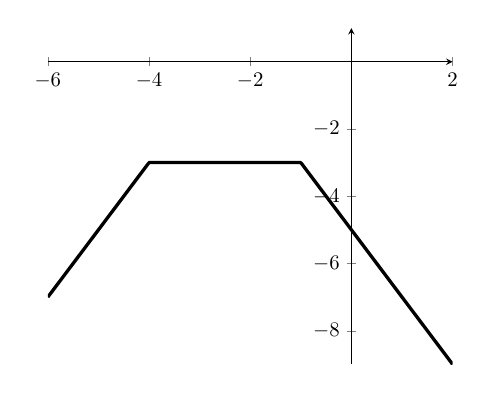
\begin{tikzpicture}[scale=0.75]
\begin{axis}[
        axis x line=middle, 
        axis y line=middle, 
        ymax=1, 
        %ymin=-4
        ]        
    \addplot[domain=-6:2, samples=400, black, ultra thick]  {(-1)*abs(x+4) - abs(x+1)};
 \end{axis}
\end{tikzpicture} \\
\end{tabular}

\vfill

{\sc{Word Problem:}}  During a 14-year period from 1990 to 2004, the population $P$ ( in thousands) of Weest Virginia fluctuated according to the model 
$$P=0.0108t^4-.211t^3+0.40t^2+7.9t+1791, \: 1 \leq t \leq 14$$
where $t$ represents t he year. (So, $t=0$ corresponds to 1990.)\\
(i) Use the graph below to determine the years during which the population was increasing. Ask the same question for decreasing population.
(ii) Approximate the maximum population between 1990 and 2004.\\

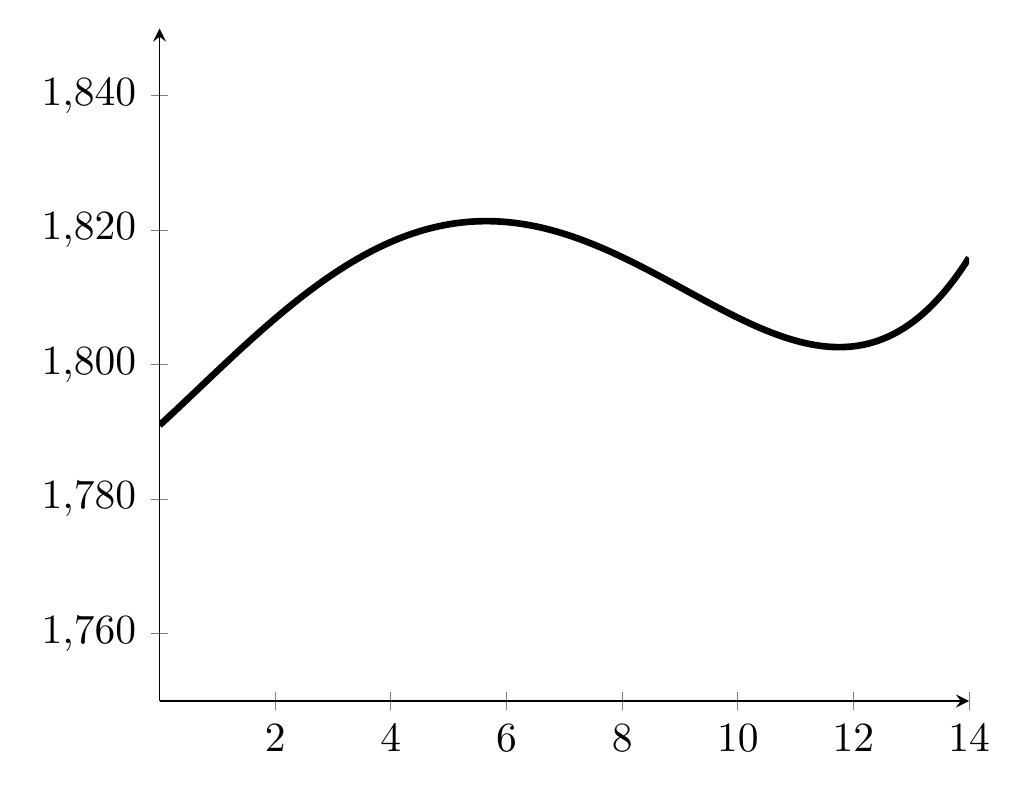
\begin{tikzpicture}[scale=1.5]
\begin{axis}[
        axis x line=middle, 
        axis y line=middle, 
        ymax=1850, 
        ymin=1750
        ]        
    \addplot[domain=0:14, samples=400, black, ultra thick]  {0.0108*x^4-.211*x^3+0.40*x^2+7.9*x+1791};
 \end{axis}
\end{tikzpicture} \\

\end{document}



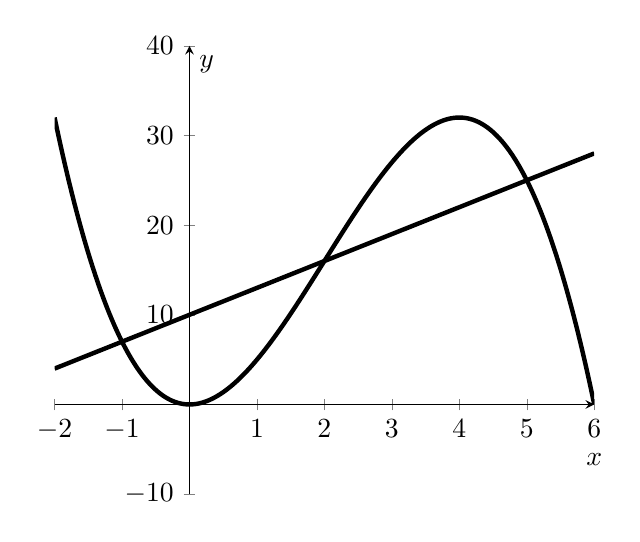
\begin{tikzpicture}[scale=1]
\begin{axis}[
        axis x line=middle, 
        axis y line=middle, 
        ymax=40, 
        ymin=-10,
        ylabel=$y$, 
        xtick={-2,-1,1,2,3,4,5,6},
        x label style={at={(current axis.right of origin)},anchor=north, below=5mm},
         xlabel=$x$,
        %x label style={at={(axis description cs:4,-1)},anchor=north},
        ]
    \addplot[domain=-2:6, samples=400, black, ultra thick]  {3*x+10};
    \addplot[domain=-2:6, samples=400, black, ultra thick]  {6*x^2-x^3};
\end{axis}
\end{tikzpicture}

